\chapter{Useful Python}

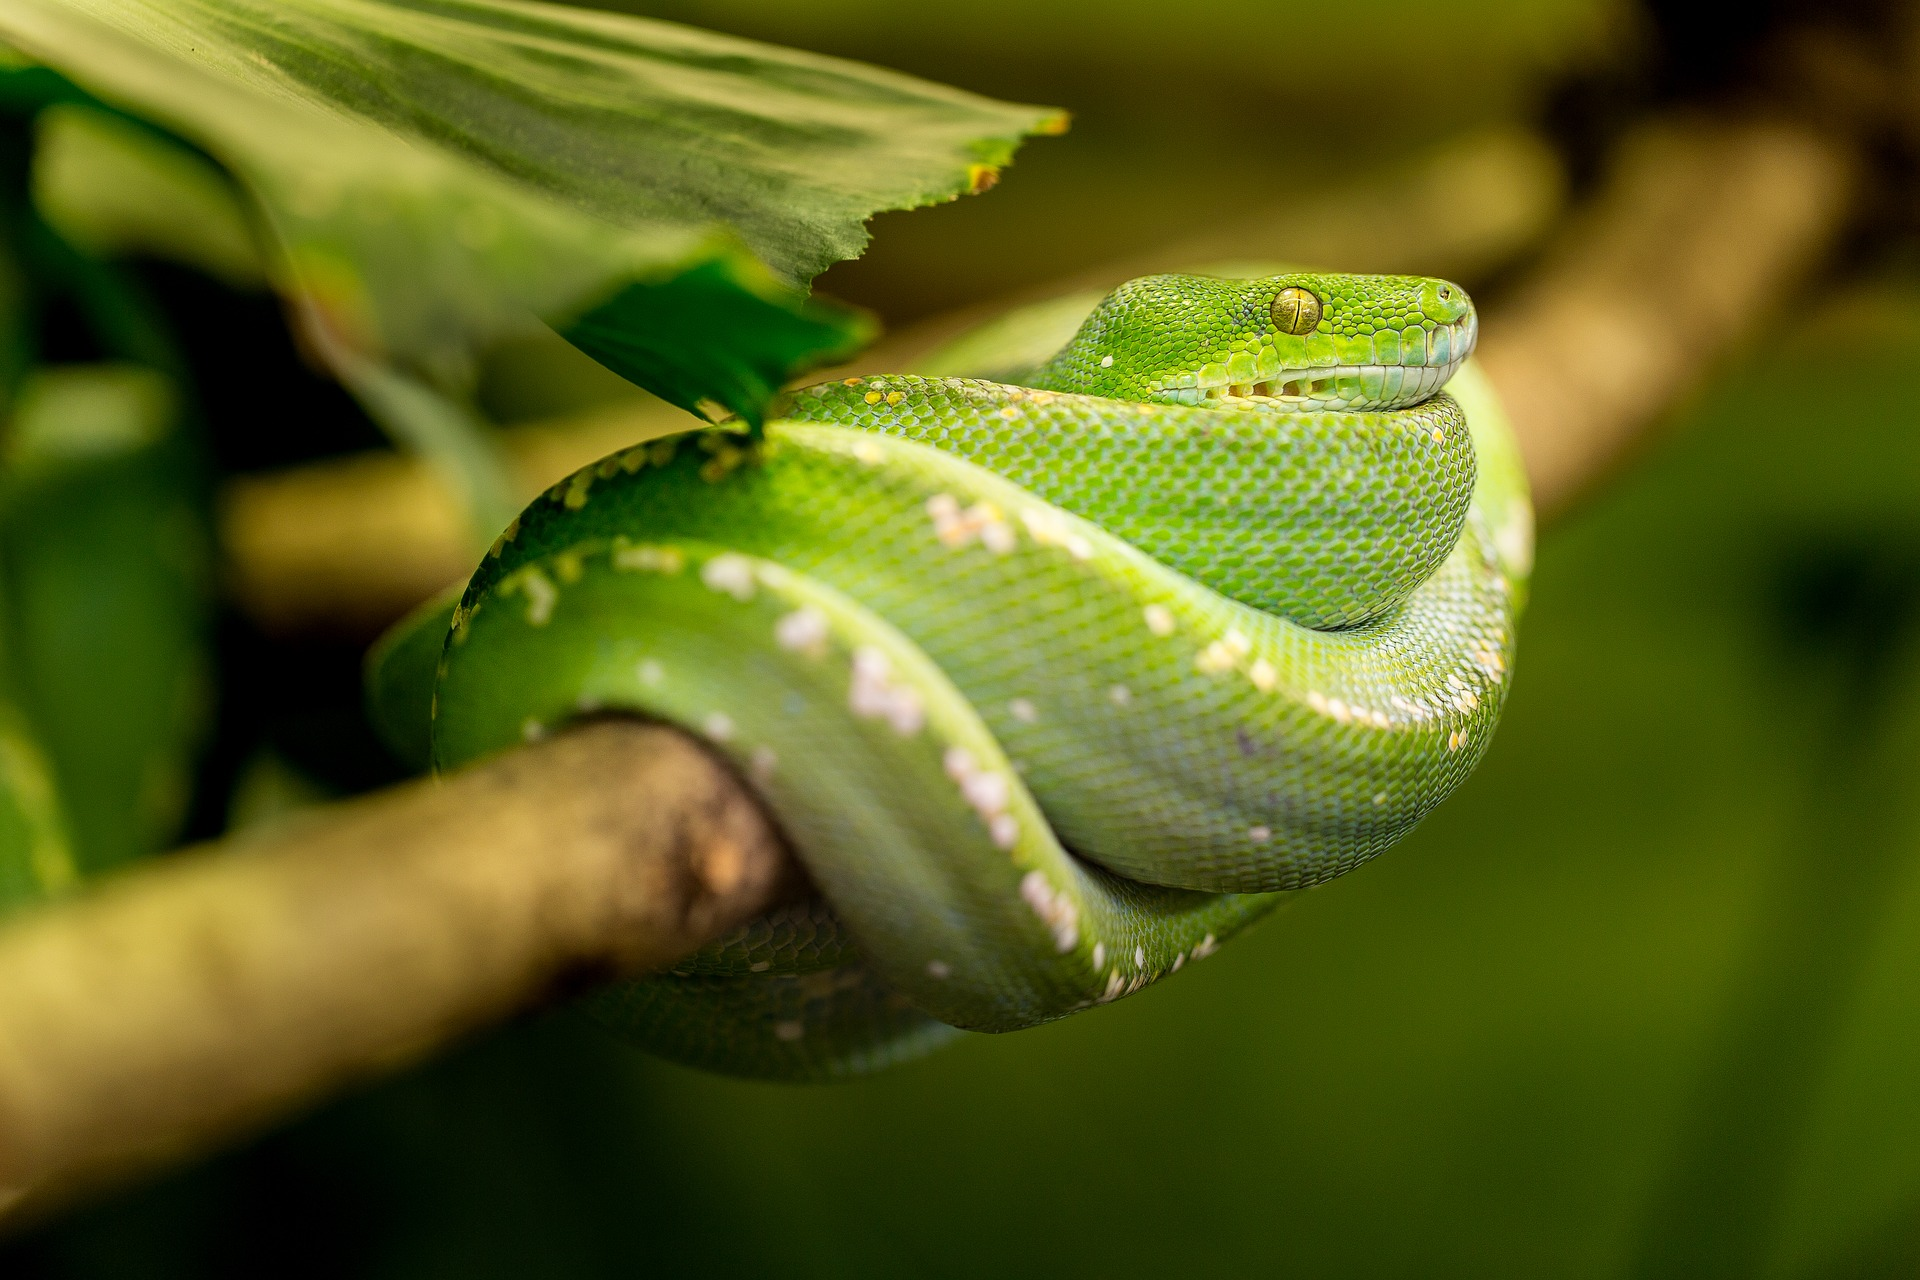
\includegraphics[scale=0.85]{images/snake-1634293_1920.jpg}

\justify{}
Getting started in writing programs is easy with Python. It is a highly 
extensible language, since there are many add on modules available. 
There is a collection known as Pypi where many of these are hosted.
Python is fairly easy to learn, especially when compared to other languages.
Python runs ``everywhere'', for all intents and purposes. For all these reasons,
Python is a great choice.

\justify{}
An item of note, Python3 is our only choice at this point. Python 2.x End of Life was
January 1st, 2020.

\section{The \_\_init\_\_.py File}

\justify{}
We add this file to let the Python interpreter know that the directories
it is found in are a contiguous part of our Python project. Since module
imports and function definitions in this file are available to all the
python code files in the directory, we can use it to our advantage. For
example, try adding this quick and dirty logging function to
python/devsecops/lib/\_\_init\_\_.py

\justify{}
\begin{mybox}{\thetcbcounter: \_\_init\_\_.py}
  \lstinputlisting{code/06-python/init.py}
\end{mybox}

\justify{}
Now we can create a Python file log\_test.py and call the logger from within like so:

\begin{mybox}{\thetcbcounter: logtest.py}
  \lstinputlisting{code/06-python/logtest.py}
\end{mybox}

\justify{}
Check the results in the file /var/log/devsecops/devsecops.log.

\section{Requirements File}

\justify{}
A requirements file under python/requirements.txt\index{requirements.txt} lists
the required Python modules needed to build and run any Python portions of our  project.
We also add a check in the Makefile to verify the existence of the requirements.txt file.
The intention is, so we can quickly cut and paste the Makefile into a new project, but
not break anything if no requirements are present yet.

\section{Test requirements}

\justify{}
Some requirements are strictly intended to be part of the test harness, but are not
needed for the application proper. Using a separate file, such as
python/requirements-test.txt, makes this delineation clear to
folks who are not familiar with the project.

\justify{}
Note that we can also include test requirements in our tox.ini file, as detailed
in the next section.

\section{Project Testing}
\justify{}
Security and reliability in our lab and rapid prototyping work is just as important as it is in our work for the Production environment. In fact, you might say it's even more important since today's rapid mock ups
can easily wind up making it into the build pipeline when folks are under a time crunch to deliver.

\justify{}
There are many test frameworks out there, lots of great ideas put forth by the community. For our current
efforts, we've settled on Tox\index{Tox} as the framework of choice. It dovetails nicely with the rest of
our patterns. Tox allows us to manage requirements for virtual environments when testing, acts as a front
end to pytest and coverage modules, and much more. It is highly configurable and extensible. For example
we can test that an application is compatible with multiple versions of Python.

\justify{}
Use the make test command inside the docker container to run the test suite for the project.

\justify{}
An example tox.ini\index{tox.ini} file follows. Take notice of the ``deps'' section,
where Python module requirements can be specified. In our current configuration,
these are in lieu of test harness requirements specified in our
python/requirements-test.txt file.

\begin{mybox}{\thetcbcounter: An example tox.ini file}
  \lstinputlisting{code/06-python/tox.ini}
\end{mybox}

\section{Test Cases}

\justify{}
Unit and functional testing is foundational in developing robust, secure
code. We want to be sure that when we create new code, we are also adding
test cases to our test suite that fully cover the new classes, functions, and so on.


\justify{}
Consider the following example unit test case. The purpose is to test
that the function check\_docker() in the file python/devsecops/lib/helper\_functions.py 
returns True when called from inside a Docker container.

\begin{mybox}{\thetcbcounter: An example Unit test case}
  \lstinputlisting{code/06-python/test-unit-example.py}
\end{mybox}

\section{Test Coverage}

\justify{}
As mentioned previously, we can avail ourselves of the coverage module by adding it to test-requirements.txt or the deps section of our tox.ini file. The purpose is to automatically generate a report on how much of
our code is ``covered'' by test cases in python/test.

\section{Python Directory Structure}
\justify{}
Files and folders relevant to the Python portions of our project are shown in the diagram below.

\begin{figure}[!htb]
  \centering
  
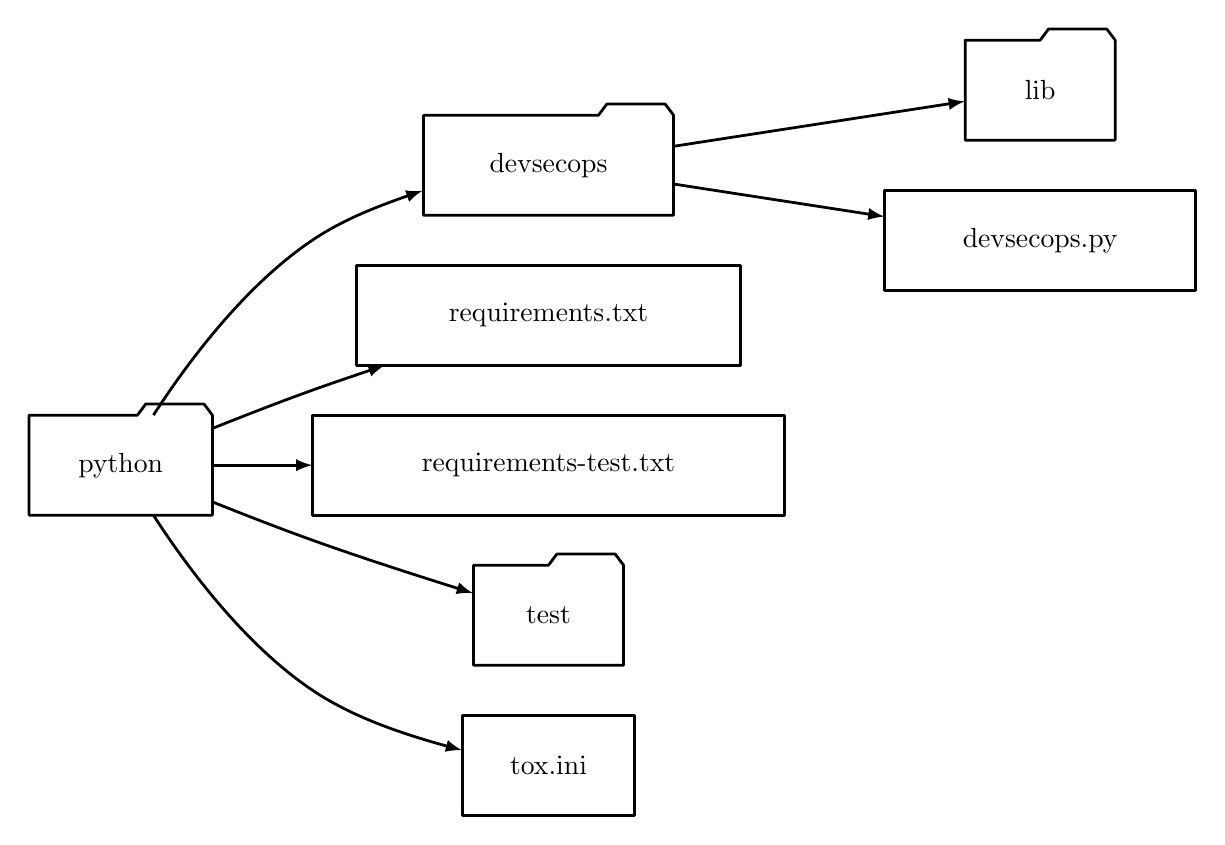
\begin{tikzpicture}[>=latex,line join=bevel,]
  \pgfsetlinewidth{1bp}
%%
\begin{scope}
  \pgfsetstrokecolor{black}
  \definecolor{strokecol}{rgb}{1.0,1.0,1.0};
  \pgfsetstrokecolor{strokecol}
  \definecolor{fillcol}{rgb}{1.0,1.0,1.0};
  \pgfsetfillcolor{fillcol}
  \filldraw (0.0bp,0.0bp) -- (0.0bp,279.0bp) -- (420.0bp,279.0bp) -- (420.0bp,0.0bp) -- cycle;
\end{scope}
\begin{scope}
  \pgfsetstrokecolor{black}
  \definecolor{strokecol}{rgb}{1.0,1.0,1.0};
  \pgfsetstrokecolor{strokecol}
  \definecolor{fillcol}{rgb}{1.0,1.0,1.0};
  \pgfsetfillcolor{fillcol}
  \filldraw (0.0bp,0.0bp) -- (0.0bp,279.0bp) -- (420.0bp,279.0bp) -- (420.0bp,0.0bp) -- cycle;
\end{scope}
\begin{scope}
  \pgfsetstrokecolor{black}
  \definecolor{strokecol}{rgb}{1.0,1.0,1.0};
  \pgfsetstrokecolor{strokecol}
  \definecolor{fillcol}{rgb}{1.0,1.0,1.0};
  \pgfsetfillcolor{fillcol}
  \filldraw (0.0bp,0.0bp) -- (0.0bp,279.0bp) -- (420.0bp,279.0bp) -- (420.0bp,0.0bp) -- cycle;
\end{scope}
\begin{scope}
  \pgfsetstrokecolor{black}
  \definecolor{strokecol}{rgb}{1.0,1.0,1.0};
  \pgfsetstrokecolor{strokecol}
  \definecolor{fillcol}{rgb}{1.0,1.0,1.0};
  \pgfsetfillcolor{fillcol}
  \filldraw (0.0bp,0.0bp) -- (0.0bp,279.0bp) -- (420.0bp,279.0bp) -- (420.0bp,0.0bp) -- cycle;
\end{scope}
\begin{scope}
  \pgfsetstrokecolor{black}
  \definecolor{strokecol}{rgb}{1.0,1.0,1.0};
  \pgfsetstrokecolor{strokecol}
  \definecolor{fillcol}{rgb}{1.0,1.0,1.0};
  \pgfsetfillcolor{fillcol}
  \filldraw (0.0bp,0.0bp) -- (0.0bp,279.0bp) -- (420.0bp,279.0bp) -- (420.0bp,0.0bp) -- cycle;
\end{scope}
  \pgfsetcolor{black}
  % Edge: py -> devsecops
  \draw [->] (44.786bp,144.03bp) .. controls (56.639bp,162.38bp) and (77.312bp,190.41bp)  .. (102.0bp,207.0bp) .. controls (111.05bp,213.08bp) and (121.57bp,217.87bp)  .. (141.58bp,224.77bp);
  % Edge: py -> req
  \draw [->] (66.002bp,139.22bp) .. controls (77.313bp,143.75bp) and (90.164bp,148.75bp)  .. (102.0bp,153.0bp) .. controls (107.23bp,154.88bp) and (112.66bp,156.76bp)  .. (127.99bp,161.91bp);
  % Edge: py -> tst
  \draw [->] (66.235bp,126.0bp) .. controls (74.043bp,126.0bp) and (82.785bp,126.0bp)  .. (101.9bp,126.0bp);
  % Edge: py -> 8
  \draw [->] (66.002bp,112.78bp) .. controls (77.313bp,108.25bp) and (90.164bp,103.25bp)  .. (102.0bp,99.0bp) .. controls (117.58bp,93.41bp) and (134.98bp,87.728bp)  .. (159.74bp,79.944bp);
  % Edge: py -> C
  \draw [->] (44.786bp,107.97bp) .. controls (56.639bp,89.621bp) and (77.312bp,61.591bp)  .. (102.0bp,45.0bp) .. controls (115.12bp,36.183bp) and (131.31bp,30.088bp)  .. (155.81bp,23.392bp);
  % Edge: devsecops -> lib
  \draw [->] (232.16bp,240.81bp) .. controls (261.43bp,245.33bp) and (299.36bp,251.18bp)  .. (336.81bp,256.96bp);
  % Edge: devsecops -> 9
  \draw [->] (232.16bp,227.19bp) .. controls (252.09bp,224.11bp) and (276.04bp,220.42bp)  .. (307.88bp,215.5bp);
  % Node: devsecops
\begin{scope}
  \definecolor{strokecol}{rgb}{0.0,0.0,0.0};
  \pgfsetstrokecolor{strokecol}
  \draw (232.0bp,252.0bp) -- (229.0bp,256.0bp) -- (208.0bp,256.0bp) -- (205.0bp,252.0bp) -- (142.0bp,252.0bp) -- (142.0bp,216.0bp) -- (232.0bp,216.0bp) -- cycle;
  \draw (187.0bp,234.0bp) node {devsecops};
\end{scope}
  % Node: 8
\begin{scope}
  \definecolor{strokecol}{rgb}{0.0,0.0,0.0};
  \pgfsetstrokecolor{strokecol}
  \draw (214.0bp,90.0bp) -- (211.0bp,94.0bp) -- (190.0bp,94.0bp) -- (187.0bp,90.0bp) -- (160.0bp,90.0bp) -- (160.0bp,54.0bp) -- (214.0bp,54.0bp) -- cycle;
  \draw (187.0bp,72.0bp) node {test};
\end{scope}
  % Node: req
\begin{scope}
  \definecolor{strokecol}{rgb}{0.0,0.0,0.0};
  \pgfsetstrokecolor{strokecol}
  \draw (256.0bp,198.0bp) -- (118.0bp,198.0bp) -- (118.0bp,162.0bp) -- (256.0bp,162.0bp) -- cycle;
  \draw (187.0bp,180.0bp) node {requirements.txt};
\end{scope}
  % Node: tst
\begin{scope}
  \definecolor{strokecol}{rgb}{0.0,0.0,0.0};
  \pgfsetstrokecolor{strokecol}
  \draw (272.0bp,144.0bp) -- (102.0bp,144.0bp) -- (102.0bp,108.0bp) -- (272.0bp,108.0bp) -- cycle;
  \draw (187.0bp,126.0bp) node {requirements-test.txt};
\end{scope}
  % Node: C
\begin{scope}
  \definecolor{strokecol}{rgb}{0.0,0.0,0.0};
  \pgfsetstrokecolor{strokecol}
  \draw (218.0bp,36.0bp) -- (156.0bp,36.0bp) -- (156.0bp,0.0bp) -- (218.0bp,0.0bp) -- cycle;
  \draw (187.0bp,18.0bp) node {tox.ini};
\end{scope}
  % Node: lib
\begin{scope}
  \definecolor{strokecol}{rgb}{0.0,0.0,0.0};
  \pgfsetstrokecolor{strokecol}
  \draw (391.0bp,279.0bp) -- (388.0bp,283.0bp) -- (367.0bp,283.0bp) -- (364.0bp,279.0bp) -- (337.0bp,279.0bp) -- (337.0bp,243.0bp) -- (391.0bp,243.0bp) -- cycle;
  \draw (364.0bp,261.0bp) node {lib};
\end{scope}
  % Node: 9
\begin{scope}
  \definecolor{strokecol}{rgb}{0.0,0.0,0.0};
  \pgfsetstrokecolor{strokecol}
  \draw (420.0bp,225.0bp) -- (308.0bp,225.0bp) -- (308.0bp,189.0bp) -- (420.0bp,189.0bp) -- cycle;
  \draw (364.0bp,207.0bp) node {devsecops.py};
\end{scope}
  % Node: py
\begin{scope}
  \definecolor{strokecol}{rgb}{0.0,0.0,0.0};
  \pgfsetstrokecolor{strokecol}
  \draw (66.0bp,144.0bp) -- (63.0bp,148.0bp) -- (42.0bp,148.0bp) -- (39.0bp,144.0bp) -- (0.0bp,144.0bp) -- (0.0bp,108.0bp) -- (66.0bp,108.0bp) -- cycle;
  \draw (33.0bp,126.0bp) node {python};
\end{scope}
%
\end{tikzpicture}


  \caption{Project Directory and related files.}
\label{pythonfiles}
\end{figure}